\documentclass[12pt,a4paper]{article}
\synctex=1
\usepackage[utf8]{inputenc}
\usepackage[margin=1cm]{geometry}
\usepackage{graphicx}
%\usepackage{verbatim}
\usepackage{amsmath}
\usepackage{amsfonts}
\usepackage{amssymb}
\usepackage{listings}
\usepackage{enumitem}
\usepackage{textcomp}
\usepackage{courier}
\usepackage{libertine}
\usepackage{pgfornament}
\usepackage{eso-pic}
\usepackage[hangul]{kotex}
\linespread{1.3}

\title{
	\centering
	\pgfornament[width=12cm,color=teal]{84}\\
	\vspace{1cm}
	\fontsize{50}{50} \selectfont {정보통신 수학 및 실습\\3월 3주차 Lab assignment}\\
		\pgfornament[width=12cm,color=teal]{88}\\
	\vfill}
\author{
	\LARGE
	\begin{tabular}{rl}
		\hline
		학번 : & 2016110056\\ 
		학과 : & 불교학부 \\
		이름 : & 박승원\\
		날짜 : & \today\\
		\hline
	\end{tabular}\vspace{1cm}
	\\

\includegraphics[width=0.5\textwidth]{logo.jpg}
	}
\date{}

\begin{document}
\maketitle
\pagenumbering{gobble}
\noindent
\lstset{language=matlab, columns=flexible, tabsize=4, frame=shadowbox, showstringspaces=false, breaklines=true, upquote=true, basicstyle=\normalsize}

\renewcommand{\thesubsubsection}{\alph{subsubsection})}
\renewcommand{\thesubsection}{\arabic{subsection}.}
\newpage
\section*{Chapter 1. Lab Assignment}

\subsection {Solve the following problems using MATLAB when:}
$f(x) = 5x^2-3x+1$\\
f = [5,-3,1]\\

\subsubsection{Evaluate f(x) for x= -1, 0, 1} 

x=[-1:1]\\
polyval(f,x)\\
ans =

9   1   3




\subsubsection{Find the roots of f(x)} 

roots(f)\\
ans =

0.30000 + 0.33166i\quad0.30000 - 0.33166i


\subsubsection{Factorize the f(x) using (b)} 

5(x-(0.3+0.33166i))(x-(0.3-0.33166i))

\subsubsection{Express x whose values are between -1 and 1 and stepping interval of 0.1.} 

x=[-1:0.1:1]

\subsubsection{Evaluate f(x) for the x values defined in (d).} 

y = polyval(f,x)

ans =

Columns 1 through 10:\\
9.00000   7.75000   6.60000   5.55000   4.60000   3.75000   3.00000   2.35000   1.80000   1.35000

Columns 11 through 20:\\
1.00000   0.75000   0.60000   0.55000   0.60000   0.75000   1.00000   1.35000   1.80000   2.35000

Column 21:\\
3.00000

\subsubsection{Plot f(x) in (e).  Label the x-axis as “X” and the y-axis “F(x)”.  Turn the grid on.} 
plot(x, y), xlabel('X'), ylabel('F(x)'), grid

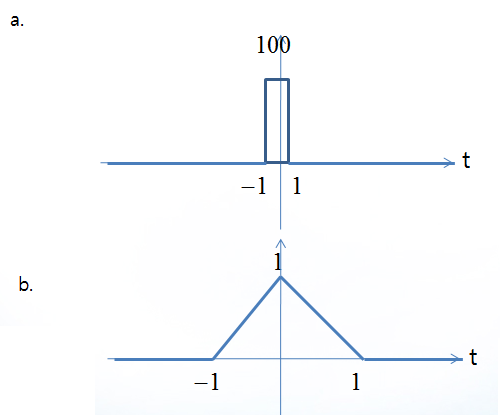
\includegraphics[width=\textwidth]{1.png}


\subsection{Compute the following problems using MATLAB when:} 


\subsubsection{Express f(x) and g(x) in MATLAB.} 

$f(x) = x^2-5x+1\\
g(x) = x^2-3x+7$

f = [1,-5,1]\\
g = [1,-3,7]

\subsubsection{Compute h(x) = f(x)*g(x)} 

h = conv(f,g)\\
ans = 1   -8   23  -38    7\\
$\Longrightarrow x^4-8x^3+23x^2-38x+7$

\subsubsection{Compute h(x) = f(x)/g(x)} 

[a,b] = deconv(f, g)\\
a =  1\\
b =\\
0  -2  -6\\
$\Longrightarrow f(x) = 1\times g(x) -2x-6$


\end{document}
